\documentclass[a4paper]{article}
\usepackage[utf8x]{inputenc}
\usepackage[T1,T2A]{fontenc}
\usepackage[russian]{babel}
\usepackage{hyperref}
\usepackage{indentfirst}
\usepackage{listings}
\usepackage{color}
\usepackage{here}
\usepackage{array}
\usepackage{multirow}
\usepackage{graphicx}

\usepackage{caption}
\renewcommand{\lstlistingname}{Программа} % заголовок листингов кода

\usepackage{listings}
\lstset{ %
extendedchars=\true,
keepspaces=true,
language=bash,					% choose the language of the code
basicstyle=\footnotesize,		% the size of the fonts that are used for the code
numbers=left,					% where to put the line-numbers
numberstyle=\footnotesize,		% the size of the fonts that are used for the line-numbers
stepnumber=1,					% the step between two line-numbers. If it is 1 each line will be numbered
numbersep=5pt,					% how far the line-numbers are from the code
backgroundcolor=\color{white},	% choose the background color. You must add \usepackage{color}
showspaces=false				% show spaces adding particular underscores
showstringspaces=false,			% underline spaces within strings
showtabs=false,					% show tabs within strings adding particular underscores
frame=single,           		% adds a frame around the code
tabsize=2,						% sets default tabsize to 2 spaces
captionpos=b,					% sets the caption-position to bottom
breaklines=true,				% sets automatic line breaking
breakatwhitespace=false,		% sets if automatic breaks should only happen at whitespace
escapeinside={\%*}{*)},			% if you want to add a comment within your code
postbreak=\raisebox{0ex}[0ex][0ex]{\ensuremath{\color{red}\hookrightarrow\space}}
}

\usepackage[left=2cm,right=2cm,
top=2cm,bottom=2cm,bindingoffset=0cm]{geometry}

\begin{document}	% начало документа
\begin{titlepage}
	\begin{center}
		\large Санкт-Петербургский Политехнический Университет Петра Великого\\
		\large Институт компьютерных наук и технологий \\
		\large Кафедра компьютерных систем и программных технологий\\[6cm]
		\huge Программирование\\[0.5cm]
		\large Отчет по курсовой работе\\[0.1cm]
		\large "Умное расписание"\\[5cm]
	\end{center}

	\begin{flushright}
		\begin{minipage}{0.25\textwidth}
			\begin{flushleft}
				\large\textbf{Работу выполнил:}\\
				\large Дьячков В.В.\\
				\large {Группа:} 23501/4\\
				\large \textbf{Преподаватель:}\\
				\large Вылегжанина К.Д.
			\end{flushleft}
		\end{minipage}
	\end{flushright}
	\vfill
	\begin{center}
	\large Санкт-Петербург\\
	\large \the\year
	\end{center}

\thispagestyle{empty}
\end{titlepage}

\vfill

% Содержание
\tableofcontents
\newpage



\section{Приложение Smart Schedule}

В наше время важным навыком стало умение грамотно распределять свое время. Особенно часто с такой задачей сталкиваются учащиеся: студенты и школьники. Оптимальным решением в данном случае может стать ведение учебного расписания и учет заданий, которые необходимо выполнить. Таким образом, было принято решение создать приложение \texttt{Smart Schedule}, предоставляющее пользователю данную функциональность.

\subsection{Задание}

Реализовать приложение на Java, которое позволяет вводить и просматривать учебное расписание и домашние задания, необходимые выполнить к определенной дате.

\subsection{Концепция приложения Smart Schedule}

Созданное приложение должно давать пользователю возможность ведения интерактивного расписания с возможность добавления, изменения и удаления занятий из расписания. Другой важно функциональностью является работа с заданиями, а именно их добавление, редактирование и удаление. Также расписание должно обладать графическим интерфейсом, который позволит визуализировать заявленную функциональность и упростить общение с программой.

\subsection{Минимально работоспособный продукт}

Консольное приложение, позволяющее пользователю вводить и просматривать учебное расписание и домашние задания.

\subsection{Диаграмма прецедентов использования}

\begin{figure}[H]
	\begin{center}
		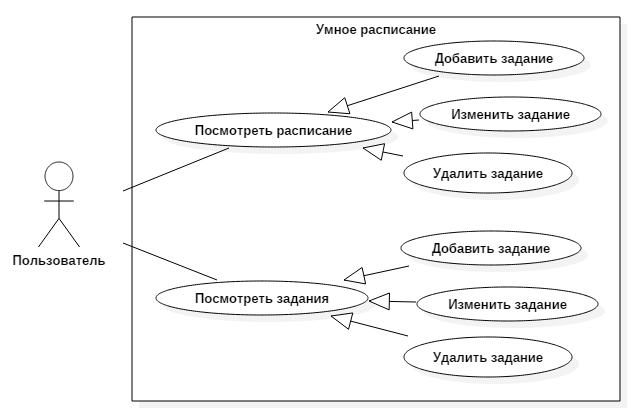
\includegraphics[scale=0.7]{pics/usecase}
		\caption{Диаграмма прецедентов использования} 
		\label{pic:use_case_diagram} % название для ссылок внутри кода
	\end{center}
\end{figure}

Выше на рис. \ref{pic:use_case_diagram} показана диаграмма прецедентов использования умного расписания. Пользователь может работать с расписанием: добавлять, изменять и удалять занятия, а также работать с заданиями: добавлять, изменять и удалять задания.

\subsection{Выводы}
В данном разделе было определены требования к приложению \texttt{Smart Schedule}, его концепция, диаграмма прецедентов использования приложения и минимально работоспособный продукт.

\section{Проектирование приложения Smart Schedule}

В процессе проектирования было решено выделить 3 подпроекта:
\begin{enumerate}
\item \texttt{core} -- библиотека, содержащая всю бизнес-логику приложения;
\item \texttt{cli} -- консольное приложение, позволяющее взаимодействовать пользователю с библиотекой через командную строку;
\item \texttt{desktop} -- графическое приложение, позволяющее взаимодействовать пользователю с библиотекой через графический интерфейс. Создано с использованием библиотеки JavaFX.
\end{enumerate}

\subsection{Диаграмма компонентов}

\begin{figure}[H]
	\begin{center}
		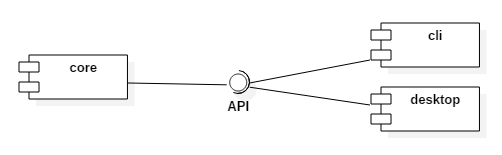
\includegraphics[scale=0.8]{pics/components}
		\caption{Диаграмма компонентов} 
		\label{pic:component_diagram}
	\end{center}
\end{figure}

Выше на рис. \ref{pic:component_diagram} представлена диаграмма компонентов, где \texttt{core} -- библиотека, \texttt{cli} -- консольное приложение и \texttt{desktop} -- графическое приложение.

\subsection{Интерфейс библиотеки}

Библиотека, представленная подпроектом \texttt{core}, содержит все необходимые классы для добавления, хранения, изменения и добавления занятий и заданий. В \texttt{API} приложения было решено выделить следующие методы:

\begin{enumerate}

    \item Получить расписание на текущую неделю

    \verb+StudySchedule getCurrentSchedule();+


    \item Получить расписание на заданную неделю

    \verb+StudySchedule getSchedule(WeekType typeOfWeek);+


    \item Поменять местами порядок расписаний (четная - нечетная)

    \verb+void swapSchedules();+


    \item Получить текущую учебную неделю, содержащую учебные дни

    \verb+StudyWeek getCurrentWeek();+


    \item Получить заданную учебную неделю, содержащую учебные дни

    \verb+StudyWeek getWeek(WeekTime week);+


    \item Получить учебные задания

    \verb+StudyTasks getTasks();+


    \item Получить тип недели

    \verb+WeekType getWeekType(WeekTime week);+

    
    \item Обновить информацию о занятиях

    \verb+void updateLessons();+
    
\end{enumerate}

\subsection{Хранение данных}
В процессе проектирования приложения было решено использовать базу данных для хранения пользовательской информации, а именно информации о занятиях и заданиях. Было выбрано  облочное \texttt{JSON} объектно-ориентированное \texttt{NoSQL} хранилище \texttt{Orchestrate}\footnote{https://orchestrate.io/}. 

\subsection{Выводы}
В данной главе было рассмотрено проектирование умного расписания: деление на подпроекты \texttt{core}, \texttt{cli} и \texttt{desktop}, определение диаграммы компонентов, выделение основных методов интерфейса, а также принятно решение об использовании базы данных \texttt{Orchestrate}.

\section{Реализация приложение Smart Schedule}

\subsection{Среда разработки}

В процессе разработки использовалась интегрированная среда разработки \texttt{IntelliJ IDEA 2016 3.1} от компании \texttt{JetBrains}. Для сборки проекта использовалась система автоматической сборки \texttt{Gradle 3.1}. Был выбран уровень языка Java \texttt{1.8}.

\subsection{Реализация библиотеки}
В процессе разработки были выделены следующие классы, перечисления и интерфейсы, определенные в подпроекте \texttt{core}:
\begin{itemize}
\item \verb+SmartSchedule+ -- интерфейс, представляющий \texttt{API} библиотеки;
\item \verb+SmartScheduleImpl+ -- класс, реализующий интерфейс \texttt{SmartSchedule};
\item \verb+LessonType+ -- перечисление типов занятий, таких как лекция, упраженения и др.;
\item \verb+Lesson+ -- класс, инкапсулирующий в себе информацию о занятии;
\item \verb+LessonChanges+ -- перечисление возможных изменений в расписании: добавление урока, изменение существующего урока и удаление урока;
\item \verb+ChangedLesson+ -- класс, расширяющий класс \texttt{Lesson} информацией об изменении в расписании;
\item \verb+StudySchedule+ -- класс, для представления недельного расписания на четную и нечетеную недели;
\item \verb+StudyDay+ -- класс, для представления учебного дня, инкапсулирующего в себе список занятий и конкретную дату;
\item \verb+StudyWeek+ -- класс, для представления учебной недели, в отличии от \texttt{StudySchedule} характеризующейся конкретными датами и изменениями в расписании;
\item \verb+Task+ -- класс, инкапсулирующий в себе информацию о задании;
\item \verb+StudyTasks+ -- класс, для представления списка заданий, инкапсулирующий в себе список заданий;
\item \verb+Database+ -- интерфейс взаимодействия классов библиотеки с базой данных;
\item \verb+OrchestrateDB+ -- класс, реализующий интерфейс \texttt{Database} и предоставлявший доступ к базе данных Orchestrate.
\end{itemize}

\subsection{Реализация консольного приложения}

Консольное приложение, определенное в подпроекте \texttt{cli}, создано исключительно в целях ручного частичного тестирования библиотеки в процессе разработки библиотеки и ввиду этого предоставляет лишь ограниченную функциональность.

\subsection{Реализация графического приложения} 

Для реализации графического приложения, определенного в подпроекте \texttt{desktop}, была выбрана платформа \texttt{JavaFX 8}, выпущенная в 2014 году и ставшая частью пакетов JRE/JDK в \texttt{Java 8}.

JavaFX — платформа для создания desktop-приоложений, позволяет строить унифицированные приложения с насыщенным графическим интерфейсом.

\subsection{Снимки экранов пользовательского интерфейса}
\subsubsection{Командная строка}

\begin{figure}[H]
	\begin{center}
		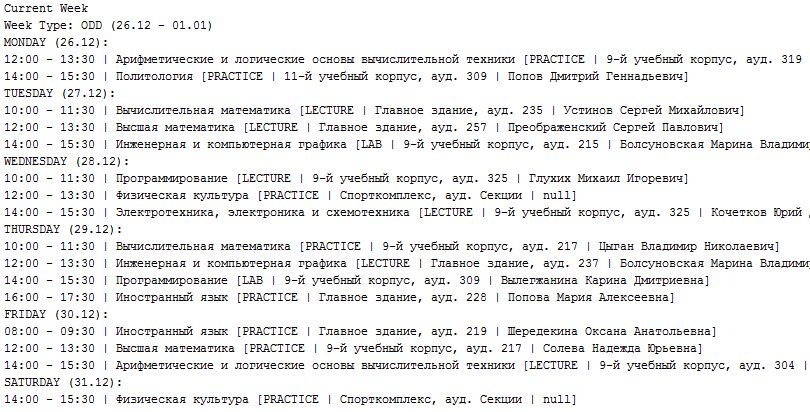
\includegraphics[scale=0.8]{pics/1}
		\caption{Расписание} 
		\label{pic:1} % название для ссылок внутри кода
	\end{center}
\end{figure}
На рис. \ref{pic:1} представлено расписание занятий.

\begin{figure}[H]
	\begin{center}
		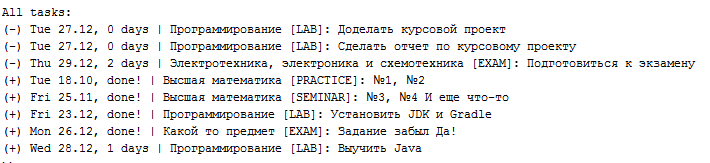
\includegraphics[scale=0.8]{pics/2}
		\caption{Список заданий} 
		\label{pic:2} % название для ссылок внутри кода
	\end{center}
\end{figure}
На рис. \ref{pic:2} представлен список заданий.

\begin{figure}[H]
	\begin{center}
		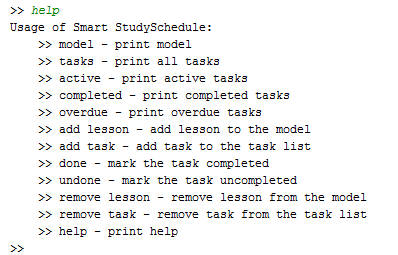
\includegraphics[scale=0.8]{pics/3}
		\caption{Список консольных команд} 
		\label{pic:3} % название для ссылок внутри кода
	\end{center}
\end{figure}
На рис. \ref{pic:3} представлен список консольных команд.


\subsubsection{Графический интерфейс}

\begin{figure}[H]
	\begin{center}
		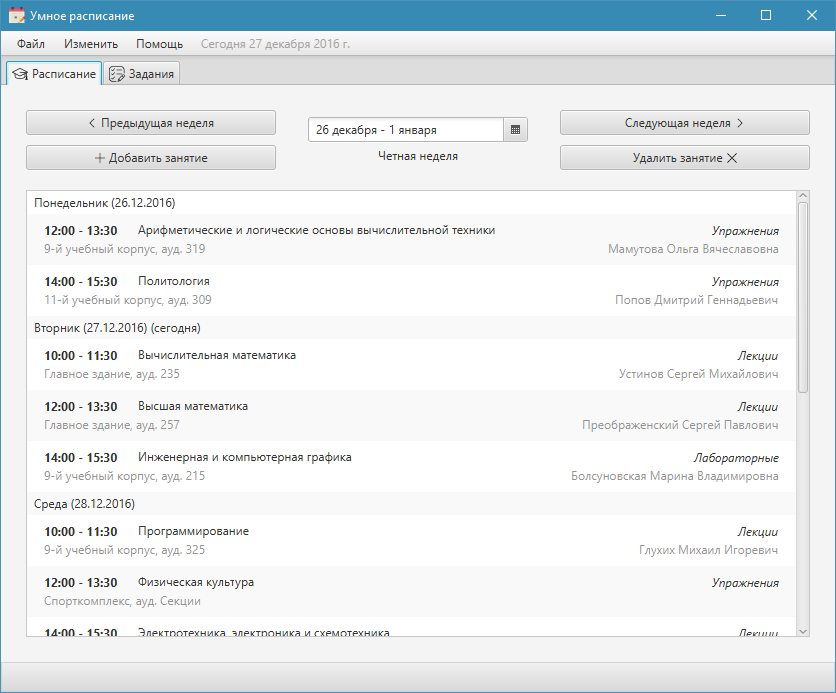
\includegraphics[scale=0.8]{pics/4}
		\caption{Расписание} 
		\label{pic:4} % название для ссылок внутри кода
	\end{center}
\end{figure}
На рис. \ref{pic:4} показано расписание. Пользователь также может перейти к предыдущей или следующей неделе, удалить или добавить задание с помощью соответствующих кнопок, а также перейти к конкретной дате с помощью календаря, расположенного в середине окна. При двойном клике на занятии появляется окно редактирования (см рис. \ref{pic:6}.

\begin{figure}[H]
	\begin{center}
		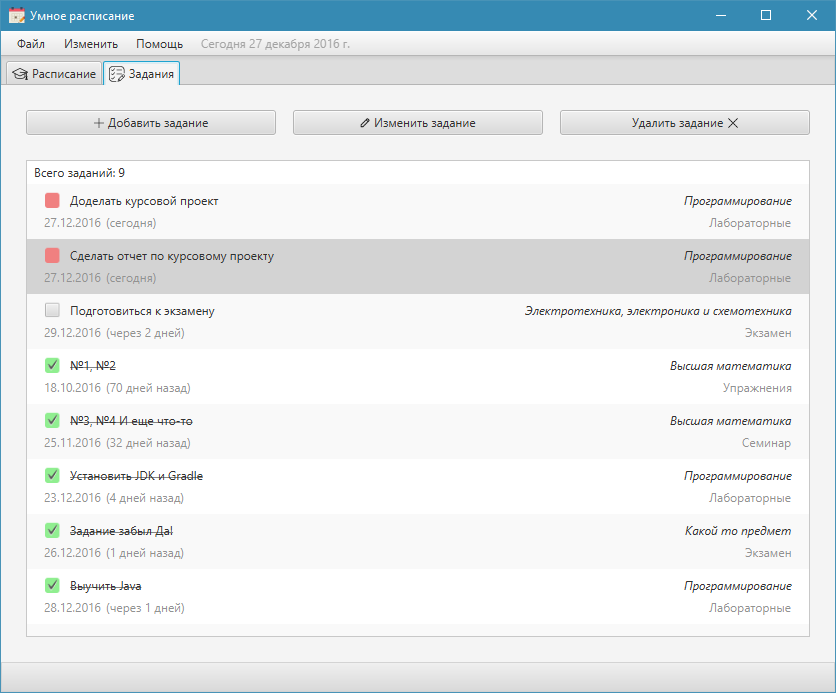
\includegraphics[scale=0.8]{pics/5}
		\caption{Список заданий} 
		\label{pic:5} % название для ссылок внутри кода
	\end{center}
\end{figure}
На рис. \ref{pic:5} показан список заданий. Пользователь может добавить, изменить или удалить задание с помощью соответствуюших кнопок. При двойном клике на задании появляется окно редактирования (см рис. \ref{pic:7}.

\begin{figure}[H]
	\begin{center}
		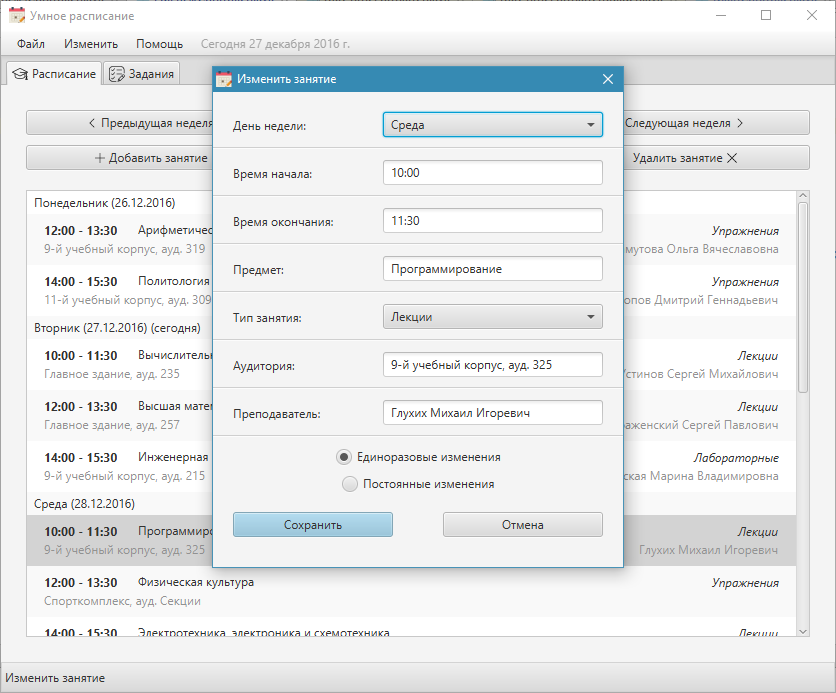
\includegraphics[scale=0.8]{pics/6}
		\caption{Редактирование занятия} 
		\label{pic:6} % название для ссылок внутри кода
	\end{center}
\end{figure}
На рис. \ref{pic:6} показано редактирование занятия. Пользователь может изменить день недели, время начала и окончания, предмет, тип занятий, аудиторию или преподавателя. Также пользователю необходимо выбрать: является ли данное изменение единоразовым (то есть изменение на конкретной неделе, в конкретный день -- в данном случае 28.12.2016) или же постоянным (то есть изменение в расписании).

\begin{figure}[H]
	\begin{center}
		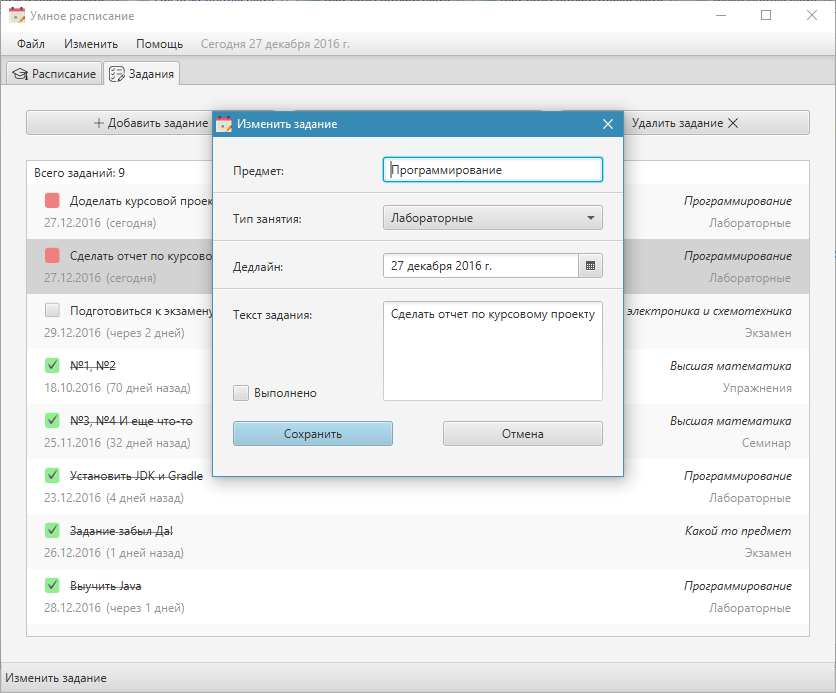
\includegraphics[scale=0.8]{pics/7}
		\caption{Редактирование задания} 
		\label{pic:7} % название для ссылок внутри кода
	\end{center}
\end{figure}
На рис. \ref{pic:6} показано редактирование задания. Пользователь может изменить предмет, по которому задано задание, тип занятия, дедлайн (дата, к которой необходимо выполнить задание) или текст задания. Также пользователь может отметить выполнение задания.

\subsection{Выводы}

В данной главе была рассмотрена реализация приложения Smart Schedule, рассмотрены основные классы библиотеки, рассмотрена реализация консольного и графического приложения, а также приведены снимки экрана работающего приложения.

\newpage
\section{Процесс обеспечения качества и тестирование}

\subsection{Утилиты и плагины}

В процессе использовались множество утилит и плагнов, таких как:
\begin{itemize}

\item Statistic\footnote{\url{https://plugins.jetbrains.com/idea/plugin/4509-statistic}}:
\begin{figure}[H]
	\begin{center}
		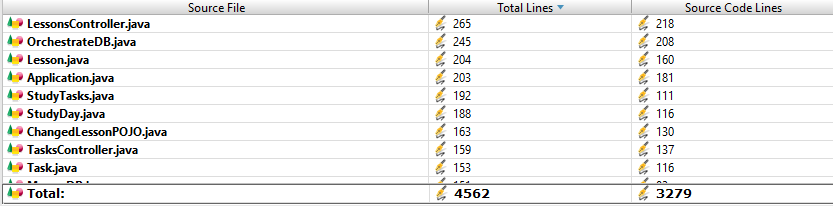
\includegraphics[scale=0.75]{pics/statistic}
		\caption{Подсчет строк кода} 
		\label{pic:statistic} % название для ссылок внутри кода
	\end{center}
\end{figure}
Statistic -- плагин для IntelliJ IDEA, предназначенный для подсчета строк кода;

\item Coverage:
\begin{figure}[H]
	\begin{center}
		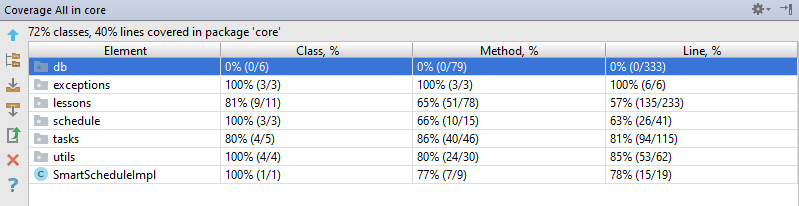
\includegraphics[scale=0.75]{pics/coverage}
		\caption{Подсчет покрытия библиотеки тестами} 
		\label{pic:coverage} % название для ссылок внутри кода
	\end{center}
\end{figure}
Coverage -- встроенное в IntelliJ IDEA средство для определения процента покрытия кода тестами;

\item FindBugs\footnote{\url{https://plugins.jetbrains.com/idea/plugin/3847-findbugs-idea}}:
\begin{figure}[H]
	\begin{center}
		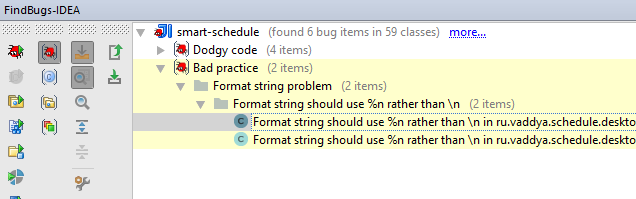
\includegraphics[scale=0.8]{pics/findbugs}
		\caption{Анализ кода} 
		\label{pic:findbugs} % название для ссылок внутри кода
	\end{center}
\end{figure}

FindBugs -- плагин для IntelliJ IDEA, предназначенный для статического анализа кода и способный обнаружить ряд ошибок, связанных со стилем кода и производительностью;

\end{itemize}

\subsection{Непрерывная интеграция}

В процессе работы использовались системы непрерывной интеграции Jenkins и Travis CI.

\textbf{Непрерывная интеграция} (англ. Continuous Integration, далее CI) — это практика разработки программного обеспечения, которая заключается в выполнении частых автоматизированных сборок проекта для скорейшего выявления и решения проблем интеграции результатов работы нескольких разработчиков. С помощью интеграционных сборок можно избавиться от синдрома «не знаю, на моей машине всё работает». Также мы защищаемся от «плохого кода», часто повторяющихся багов, «кривых» слияний. CI увеличивает возможности обратной связи потому, что она позволяет следить за состоянием проекта в течение разработки.\footnote{\url{https://ru.wikipedia.org/wiki/Continuous_integration}}

Сборка проекта и запуск тестов в Jenkins осуществлялись посредством инструмента Docker. Для этого использовался готовый контейнер\footnote{\url{https://hub.docker.com/r/lamtev/java/}}, созданный А.Ю. Ламтевым. Данный контейнер удобен тем, что содержит все необходимые компоненты среды. Для Travis CI использовалось окружение Java и OracleJDK 8. При каждом обновления репозитория производилась полная сборка проекта, его тестирование и статический, а также собиралась различная статистическая информация. Использование непрерывной интеграции позволило контролировать состояние проекта на всем протяжении разработки.  

\subsection{Просмотр кода и демонстрации}

В ходе написания приложения производился просмотр кода (code review), не участвующими в его создании людьми. Так, в ходе разработки было проведено 2 просмотра, нацеленных на выявление ошибок и недоработок, связанных  непосредственно с кодом, его стилем и архитектурой приложения. Первый просмотр был проведен 02.11.2016 Лежениным Ю.И., второй - 15.12.2016 Вылегжаниной К.Д. В ходе данных проверок было получено большое количество различных замечаний, часть из которых в итоге были исправлены.

\begin{figure}[H]
	\begin{center}
		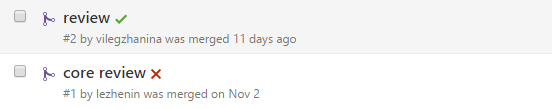
\includegraphics[scale=0.85]{pics/review}
		\caption{Просмотр кода} 
		\label{pic:findbugs} % название для ссылок внутри кода
	\end{center}
\end{figure}

В течении семестра была сделана только одна демонстрация, что несомненно сказалось в худшую сторону на приложение. Тем не менее теперь я понял значимость и необходимость проведения демонстраций в процессе работы.

\subsection{Тестирование}

\begin{figure}[H]
	\begin{center}
		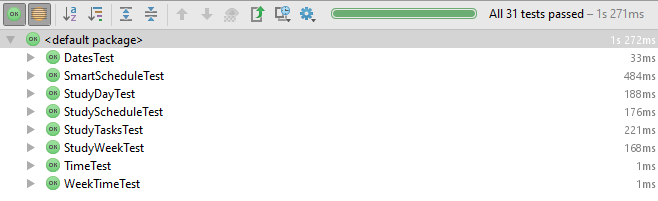
\includegraphics[scale=0.7]{pics/tests}
		\caption{Результаты тестов} 
		\label{pic:tests} % название для ссылок внутри кода
	\end{center}
\end{figure}

При разработке приложения были написаны автоматические тесты при помощи фреймворка \texttt{JUnit~4.12}, который упрощает написание тестирующего кода, целью которых было выявить некорректное поведение библиотеки. Кроме того, для написания тестов использовалась mock-библиотека \texttt{PowerMock 1.6.5}, позволяющая подменять возвращаемые значения в процессе выполнения тестов. Данная возможность позволила использовать класс-заглушку для базы данных и запустить множество тестовых сценариев.

\subsection{Выводы}

В данной главе были рассмотрены используемые в процессе разработки утилиты и плагины для среды разработки \texttt{IntelliJ IDEA}, оценен вклад просмотра кода и демонстраций, оценена полезность практики непрерывной интеграции, а также сделаны выводы о тестировании приложения.

\section{Выводы}

При выполнении задания были закреплены навыки в работе с объектно-ориентированным программированием, получен опыт в организации и разработке проекта на языке \texttt{Java}, создании и автоматизации модульных тестов, а также в использовании утилит и плагинов для интегрированной среды разработки, помогающих в разработке приложений.

Огромный шаг вперед сделан в плане практических навыков программирования и проектировании приложения.

Результатом работы стало приложение на Java, которое позволяет вводить и просматривать учебное расписание и домашние задания, необходимые выполнить к определенной дате.

\end{document}
